

\tikzset{%
  client/.style={
    rectangle,
    thick,
    draw,
    minimum size=0.7cm,
    text width=1cm,
    align=center
  },
  client missing/.style={
    draw=none, 
    scale=2,
    text height=0.333cm,
    execute at begin node=$\cdots$
  },
}


\begin{document}

%----------------------------------------------------------------------------------------
%	TITLE PAGE
%----------------------------------------------------------------------------------------

\title[联邦学习]{\huge{联邦学习中的优化问题}  \\
\medskip
\small{Optimizations in Federated Learning}
} % The short title appears at the bottom of every slide, the full title is only on the title page

% \author[文豪]{文豪} % Your name

% \institute[北京航空航天大学] % Your institution as it will appear on the bottom of every slide, may be shorthand to save space
% {
% 数学科学学院 \\ % Your institution for the title page
% \medskip
% \textit{wenh06@gmail.com} % Your email address
% 北京航空航天大学 \\
% 数学科学学院 \qquad 北京航空航天大学
% }

% \logo{\includegraphics[height=1.5cm]{logo}}
% \logoii{\includegraphics[height=1cm]{logo2}}

% \date{\footnotesize 2021年4月13日} % Date, can be changed to a custom date

\setlength{\belowdisplayskip}{5pt} \setlength{\belowdisplayshortskip}{5pt}
\setlength{\abovedisplayskip}{5pt} \setlength{\abovedisplayshortskip}{5pt}

%------------------------------------------------

\begin{frame}
\titlepage % Print the title page as the first slide
\end{frame}

%------------------------------------------------

\begin{frame}
% \frametitle{Overview} % Table of contents slide, comment this block out to remove it
\tableofcontents % Throughout your presentation, if you choose to use \section{} and \subsection{} commands, these will automatically be printed on this slide as an overview of your presentation
\end{frame}

%------------------------------------------------

%------------------------------------------------
%	PRESENTATION SLIDES
%------------------------------------------------


% PPT version (read only share link): https://www.kdocs.cn/l/cigmbsd3uAI4


%------------------------------------------------

\section{引言}

%------------------------------------------------
% Page 1

\begin{frame}
\frametitle{引言}

联邦学习(Federated Learning)来源于机器(深度)学习模型分布式(Distributed)训练的需求

\begin{figure}
    \centering
    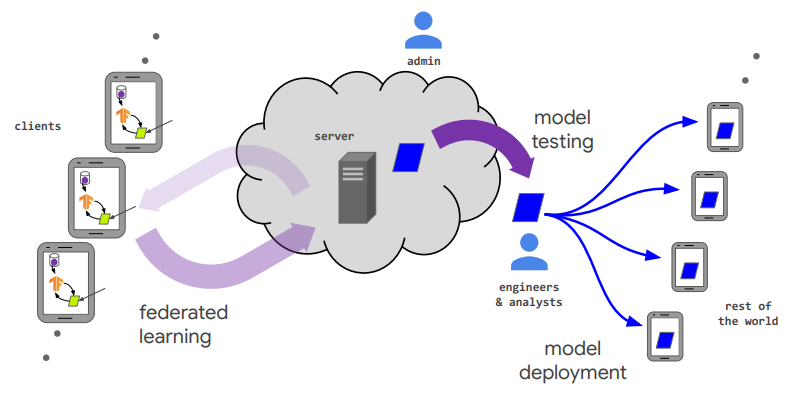
\includegraphics[width=\textwidth,keepaspectratio]{images/fl_overview.png}
\end{figure}

{\scriptsize
图片来源:\cite{kairouz2019advances_fl} Kairouz et al., Advances and open problems in federated learning, 2019
}

\end{frame}

%------------------------------------------------
% Page 15

\begin{frame}
\frametitle{引言}

这种分布式训练的需求多是当多个数据拥有方想要联合他们各自的数据训练机器学习模型,由于涉及隐私和数据安全等法律问题,或是数据庞大且过于分散导致的可行性问题,而不能将数据集中到一起进行模型训练而产生的。随着越来越严格的数据隐私方面的法律法规的施行,这种需求会越来越大。

\pause
\vspace{0.8em}

一般来说,在联邦学习的框架下,数据拥有方在不用给出己方数据的情况下,也可进行模型训练得到公共的模型$M_{fed}$,使得模型$M_{fed}$,与将数据集中到一起进行训练能得到的模型$M$,二者的预测值的偏差的期望能足够小。
$$\expectation_{z\sim\mathcal{D}} \lVert M_{fed}(z) - M(z) \rVert \leqslant \delta$$

\vspace{0.5em}

{\footnotesize 注:以下将数据拥有方统称为``节点''}

\end{frame}

%------------------------------------------------
% Page 15

\begin{frame}
\frametitle{引言}

Federated Learning这个名词首次由Google的研究人员McMahan等人在文章\cite{mcmahan2017fed_avg} \emph{Communication-Efficient Learning of Deep Networks from Decentralized Data} (2016) 中提出。

\vspace{1em}
\pause

相关的分布式的模型训练(优化)方法则可以追溯到更早的时间,例如Boyd等人的著作\cite{boyd2011distributed} \emph{Distributed Optimization and Statistical Learning via the Alternating Direction Method of Multipliers} (2010)

\end{frame}

%------------------------------------------------
% Page 15

\begin{frame}
\frametitle{联邦学习的定义}

综述文章\cite{kairouz2019advances_fl} Advances and open problems in federated learning (2019)给联邦学习下过如下的定义

\vspace{0.8em}

\begin{quote}
    ``Federated learning is a machine learning setting where multiple entities (clients) collaborate in solving a machine learning problem, under the coordination of a central server or service provider. Each client's raw data is stored locally and not exchanged or transferred; instead, focused updates intended for immediate aggregation are used to achieve the learning objective.''
\end{quote}

% \pause
% \vspace{0.5em}
% \noindent 注:没有central server的去中心化学习(decentralized learning)任务,有时候也可以在广义上被认为是联邦学习。

\end{frame}

%------------------------------------------------
% Page 15

\begin{frame}
\frametitle{联邦学习研究的一些核心的问题}

\begin{itemize}
    \item {\Large\bfseries EE (Efficiency \& Effectiveness)}
    \begin{itemize}
        \item[$\bullet$] {\large\bfseries Optimization}
        \vspace{0.5em}
        \pause
        {\pgfsetfillopacity{0.4} \footnotesize
        \item[$\bullet$] Compression
        }
    \end{itemize}
    \vspace{1em}
    {\pgfsetfillopacity{0.4} \footnotesize
    \item Privacy \& Security
    \begin{itemize}
        \item[$\bullet$] Differential Privacy (DP)
        \item[$\bullet$] Secure Multi-Party Computing (SMPC)
        \item[$\bullet$] Trusted Execution Environment (TEE)
        \item[$\bullet$] Homomorphic Encryption (HE)
    \end{itemize}
    \item Applications
    \begin{itemize}
        \item[$\bullet$] Medical
        \item[$\bullet$] Recommendation
        \item[$\bullet$] Finance
    \end{itemize}
    \item $\cdots\cdots$
    }
\end{itemize}

\end{frame}

%------------------------------------------------

\section[联邦学习中的优化]{联邦学习中的优化问题与算法}

%------------------------------------------------
% Page 15

\begin{frame}
\frametitle{问题描述}

一般来说,联邦学习中我们考虑的是如下的优化问题
\begin{align*}
    & \text{minimize} \quad f(x) = \expectation\limits_{i \sim {\mathcal{P}}} [f_i(x)] \\
    & \text{where} \quad f_i(x) = \expectation\limits_{z \sim \mathcal{D}_i} [\ell_i(x; z)]
\end{align*}
这里的$\mathcal{P}$为节点的分布,$\mathcal{D}_i$为节点$i$上 的数据分布,$\ell_i$为损失函数。

\pause
\vspace{1em}

或者更简单地,考虑如下的优化问题
\begin{align*}
    & \text{minimize} \quad f(x) = \dfrac{1}{N} \sum\limits_{i=1}^N f_i(x)
\end{align*}

\end{frame}

%------------------------------------------------
% Page 15

\begin{frame}
\frametitle{问题描述}

要注意的是,联邦学习中的``节点''(数据拥有方)意义比较宽泛,涵盖很多场景,例如
\begin{itemize}
    \item 多家医院的服务器
    % 这种情况下,数据来源(分布)可能是相同的(例如都是ImageNet),但是partition是固定的,需要区别于 datacenter 的情况
    \item 多个移动设备(edge device)
    % 这种情况下,数据来源一般是不同的
\end{itemize}

\pause
\vspace{1.5em}

前者一般被称作cross-silo,后者一般被称作cross-device。在cross-device的场景下,一般来说,通信效率才是整个系统的瓶颈所在,此外还需要考虑掉队者(stragglers)等问题。

\end{frame}

%------------------------------------------------
% Page 15

\begin{frame}
\frametitle{数据分布}

在真实场景下,各个节点上的数据的分布$\mathcal{D}_i$一般不是独立同分布的(non-IID, 或称heterogeneous)。这种数据分布的各向异性将联邦学习分为了3类

\begin{itemize}
    \item 横向联邦学习:各节点的样本重叠度{\color{red} 低},样本特征重叠度{\color{green} 高}
    \item 纵向联邦学习:各节点的样本重叠度{\color{green} 高},样本特征重叠度{\color{red} 低}
    \item 迁移联邦学习:各节点的样本重叠度{\color{red} 低},样本特征重叠度{\color{red} 低}
\end{itemize}

同一种算法(例如SVM)在不同类型的联邦学习模式下,对应的优化问题的具体形式会稍有不同。

\end{frame}

%------------------------------------------------
% Page 15

\begin{frame}
\frametitle{数据分布}

% 从左到右依次是横向联邦学习,纵向联邦学习,迁移联邦学习
\begin{columns}

\begin{column}{0.26\textwidth}
\begin{figure}
\begin{tikzpicture}
\draw (0,0) rectangle (2.8,4.5);
\node at (1.25,5.5) {横向联邦学习};
\draw[fill=pink] (0,0) rectangle (2.5,1.1) node[pos=.5] {client $i$};
\draw[fill=green] (0.2,3.3) rectangle (2.8,4.5) node[pos=.5] {client $j$};
\draw[fill=yellow] (0.3,0.9) rectangle (2.7,3.6) node[pos=.4] {client $k$};
% \draw[->] (0,-0.4) edge (10, -0.4);
\node at (1.35,-0.4) {特征维度};
\end{tikzpicture}
\end{figure}
\end{column}

\begin{column}{0.26\textwidth}
\begin{figure}
\begin{tikzpicture}
\draw (0,0) rectangle (2.8,4.5);
\node at (1.25,5.5) {纵向联邦学习};
\draw[fill=pink] (0,0) rectangle (1.1,4.2) node[pos=.5,rotate=-90] {client $i$};
\draw[fill=green] (1.4,0) rectangle (2.8,4.5) node[pos=.5,rotate=-90] {client $j$};
\draw[fill=yellow] (0.9,0.3) rectangle (1.5,4.4) node[pos=.4,rotate=-90] {client $k$};
\node at (1.35,-0.4) {特征维度};
\end{tikzpicture}
\end{figure}
\end{column}

\begin{column}{0.26\textwidth}
\begin{figure}
\begin{tikzpicture}
\draw (0,0) rectangle (2.8,4.5);
\node at (1.25,5.5) {迁移联邦学习};
\draw[fill=pink] (0,0) rectangle (0.9,1.6) node[pos=.5] {client $i$};
\draw[fill=green] (1.5,3.8) rectangle (2.8,4.5) node[pos=.5] {client $j$};
\draw[fill=yellow] (0.6,1.3) rectangle (1.7,3.9) node[pos=.4] {client $k$};
\node at (1.35,-0.4) {特征维度};
\end{tikzpicture}
\end{figure}
\end{column}

\begin{column}{0.13\textwidth}
\begin{figure}
\begin{tikzpicture}
% \coordinate (sample_node) at (0,0);
% \node[text width=1, left=0.5cm of sample_node.west] at () {样本维度};
\node[text width=12pt] () {样本维度};
\end{tikzpicture}
\end{figure}
\end{column}

\end{columns}

\end{frame}

%------------------------------------------------
% Page 15

\begin{frame}
\frametitle{数据分布}

non-IID数据分布下,算法的收敛性分析相比IID数据下要更加困难,需要更多额外的假设,对节点之间的数据分布的不同性(dissimilarity)进行定量上的限制。

\vspace{1.5em}

一般地,这种限制以gradient variance给出,例如bounded inter-client gradient variance (BCGV):
$$\expectation\limits_{i \sim {\mathcal{P}}} \lVert \nabla f_i(x) - \nabla f(x) \rVert_2^2 \leqslant \text{const} \quad \text{ for all } x$$

\end{frame}

%------------------------------------------------
% Page 15

\begin{frame}
\frametitle{联邦学习的一般性框架(流程)}

\begin{itemize}
    \item client selection
    \vspace{0.5em}
    \item parameter broadcast
    \vspace{0.5em}
    \item {\large \bfseries client computation (local parameter update)}
    \vspace{0.5em}
    \item parameter aggregation
    \vspace{0.5em}
    \item {\large \bfseries server computation (global parameter update)}
\end{itemize}

\end{frame}

%------------------------------------------------
% Page 15

% reference: FLOW - Adaptive Federated Optimization

\begin{frame}
\frametitle{联邦学习的一般性框架(流程)}

Broadcast and local update:

\vspace{2em}

\begin{figure}
\centering
\begin{tikzpicture}[]
\node[] (slide-center) {};
\node[client, above=3em of slide-center] (server) {server $x$};
\node[client, below left = 1.5cm and 3.5cm of server.south] (client-1) {client $x_1$};
\node[client, right = 0.4cm of client-1.east] (client-2) {client $x_2$};
\node[client, right = 0.4cm of client-2.east] (client-3) {client $x_3$};
\node[client missing, right = 0.1cm of client-3.east] (client-missing) {};
\node[client, right = 0.1cm of client-missing.east] (client-n) {client $x_n$};
\path[->] ([xshift=-0.5cm,yshift=-0.1cm]server.south) edge ([yshift=0.15cm]client-1.north);
\path[->] ([xshift=-0.2cm,yshift=-0.1cm]server.south) edge ([yshift=0.15cm]client-2.north);
\path[->] ([xshift=0.05cm,yshift=-0.1cm]server.south) edge ([yshift=0.15cm]client-3.north);
\path[->] ([xshift=0.4cm,yshift=-0.1cm]server.south) edge ([yshift=0.15cm]client-n.north);
\node[text width=1.2cm, align=center, right=0.3cm of client-n.east] (local-update) {local update};
\node[text width=1.8cm, align=center, above left=0.5cm and 0.3cm of local-update.north] () {params broadcast};
\end{tikzpicture}
\end{figure}

\end{frame}

%------------------------------------------------
% Page 15

% reference: FLOW - Adaptive Federated Optimization

\begin{frame}
\frametitle{联邦学习的一般性框架(流程)}

Aggregate and global update:

\vspace{2em}

\begin{figure}
\centering
\begin{tikzpicture}[]
\node[] (slide-center) {};
\node[client, above=3em of slide-center] (server) {server $x$};
\node[client, below left = 1.5cm and 3.5cm of server.south] (client-1) {client $x_1$};
\node[client, right = 0.4cm of client-1.east] (client-2) {client $x_2$};
\node[client, right = 0.4cm of client-2.east] (client-3) {client $x_3$};
\node[client missing, right = 0.1cm of client-3.east] (client-missing) {};
\node[client, right = 0.1cm of client-missing.east] (client-n) {client $x_n$};
\path[->] ([yshift=0.15cm]client-1.north) edge ([xshift=-0.5cm,yshift=-0.1cm]server.south);
\path[->] ([yshift=0.15cm]client-2.north) edge ([xshift=-0.2cm,yshift=-0.1cm]server.south);
\path[->] ([yshift=0.15cm]client-3.north) edge ([xshift=0.05cm,yshift=-0.1cm]server.south);
\path[->] ([yshift=0.15cm]client-n.north) edge ([xshift=0.4cm,yshift=-0.1cm]server.south);
\node[text width=1.2cm, align=center, right=0.3cm of server.east] (global-update) {global update};
\node[text width=1.8cm, align=center, below right=0.25cm and 0.3cm of global-update.south] () {aggregation};
\end{tikzpicture}
\end{figure}

\end{frame}

%------------------------------------------------

\section{FedOpt}  % gradient based methods

%------------------------------------------------
% Page 15

\begin{frame}
\frametitle{从FedAvg到FedOpt}

Google研究人员McMahan等人在文章\cite{mcmahan2017fed_avg}(2016)中考察了普通的SGD在分布式下的平凡推广FedSGD,即在每次循环中,节点执行一次full-batch gradient descent,并做出了进一步推广,提出了FedAvg算法。FedAvg的具体做法就是在每次循环的client local computation中,执行多步mini-batch SGD。这样,既降低了通信开销(communication-efficient),同时也在实验上观察到了模型效果的提升。

\end{frame}

%------------------------------------------------
% Page 15

\begin{frame}
\frametitle{从FedAvg到FedOpt}

\begin{algorithm}[H]
\SetAlgoNoLine
\DontPrintSemicolon
{\bfseries Server executes:}\;
\Indp initialize parameters $x_0$, learning rate $\eta$, batch size $B$;
\For{each round $t = 0, 1, \cdots, T-1$}{
    $S_t \gets$ (random set of clients)\;
    \For{each client $i \in \mathcal{S}_t$ {\bfseries in parallel}}{
        $x_{i,t} \gets$ {\bfseries ClientUpdate}$(i, x_t)$\;
        }
    $x_{t+1} \gets \frac{1}{|\mathcal{S}_t|}\sum_{i\in \mathcal{S}_t} x_{i,t}$\;
}
\Indm
\vspace{0.2em}
{\bfseries ClientUpdate}$(i, x)$: // on client $i$\;
\Indp $\mathcal{B} \gets$ (split $\mathcal{P}_i$ into batches of size $B$)\;
\For{local step $k=0,1\cdots,K-1$}{
    \For{batch $b \in \mathcal{B}$}{
        $x \gets x-\eta\nabla \ell_i(x;b)$\;
    }
}
return $x$\;
\caption{FedAvg}
\end{algorithm}

\end{frame}

%------------------------------------------------
% Page 15

\begin{frame}
\frametitle{FedSGD -- baseline}

FedSGD: 在每个节点执行一次full-batch GD之后,即进行模型同步(平均)。

\begin{figure}
\centering
\begin{tikzpicture}[]
\node[] (slide-center) {};
\node[left=9cm of slide-center] (x_t) {$x_t$};
\node[above right = 1.5cm and 0.6cm of x_t] (x_1_0) {$x_{1,t}^0$};
\node[below = 0.6cm of x_1_0] (x_2_0) {$x_{2,t}^0$};
\node[below = 0.4cm of x_2_0] (missing) {$\vdots$};
\node[below = 0.4cm of missing] (x_n_0) {$x_{n,t}^0$};
\foreach \m in {1,2,n}
{
    \path[->,brown] (x_t) edge (x_\m_0);
}

\foreach \m in {1,2,n}
{
    \node[right = 0.6cm of x_\m_0] (x_\m_1) {$x_{\m,t}^1$};
    \path[->] (x_\m_0) edge (x_\m_1);
}
\node[below right = 1.5cm and 0.6cm of x_1_1] (x_t_1) {$x_{t+1}$};
\foreach \m in {1,2,n}
{
    \path[->,green] (x_\m_1) edge (x_t_1);
}
\draw[dashed,red,thick] ([xshift=-0.7cm,yshift=0.1cm]x_1_0.north) rectangle ([xshift=0.7cm,yshift=-0.1cm]x_n_1.south);
\node[below right=0.3cm and -0.5cm of x_n_0.south] () {ONE local GD};

\node[above right = 1.5cm and 0.6cm of x_t_1] (x_11_0) {$x_{1,t+1}^0$};
\node[below = 0.6cm of x_11_0] (x_12_0) {$x_{2,t+1}^0$};
\node[below = 0.4cm of x_12_0] (missing1) {$\vdots$};
\node[below = 0.4cm of missing1] (x_1n_0) {$x_{n,t+1}^0$};
\foreach \m in {1,2,n}
{
    \path[->,brown] (x_t_1) edge (x_1\m_0);
}

\foreach \m in {1,2,n}
{
    \node[right = 0.6cm of x_1\m_0] (x_1\m_1) {$x_{\m,t+1}^1$};
    \path[->] (x_1\m_0) edge (x_1\m_1);
}
\node[below right = 1.5cm and 0.6cm of x_11_1] (x_t_2) {$x_{t+2}$};
\foreach \m in {1,2,n}
{
    \path[->,green] (x_1\m_1) edge (x_t_2);
}
\draw[dashed,red,thick] ([xshift=-0.8cm,yshift=0.1cm]x_11_0.north) rectangle ([xshift=0.8cm,yshift=-0.1cm]x_1n_1.south);
\node[below right=0.3cm and -0.5cm of x_1n_0.south] () {ONE local GD};
\end{tikzpicture}
\end{figure}

\end{frame}

%------------------------------------------------
% Page 15

\begin{frame}
\frametitle{FedAvg}

FedAvg: 每个节点执行$K$个mini-batch SGD之后,进行模型同步(平均)。在通信量大大降低的情况下,。。。。(待写)

\begin{figure}
\centering
\begin{tikzpicture}[]
\node[] (slide-center) {};
\node[left=9cm of slide-center] (x_t) {$x_t$};
\node[above right = 1.5cm and 0.8cm of x_t] (x_1_0) {$x_{1,t}^0$};
\node[below = 0.6cm of x_1_0] (x_2_0) {$x_{2,t}^0$};
\node[below = 0.4cm of x_2_0] (missing) {$\vdots$};
\node[below = 0.4cm of missing] (x_n_0) {$x_{n,t}^0$};
\foreach \m in {1,2,n}
{
    \path[->,brown] (x_t) edge (x_\m_0);
}

\foreach \m in {1,2,n}
{
    \node[right = 0.8cm of x_\m_0] (x_\m_1) {$x_{\m,t}^1$};
    \path[->] (x_\m_0) edge (x_\m_1);
}
\foreach \m in {1,2,n}
{
    \node[right = 0.8cm of x_\m_1] (x_\m_2) {$x_{\m,t}^2$};
    \path[->] (x_\m_1) edge (x_\m_2);
}
\foreach \m in {1,2,n}
{
    \node[right = 0.5cm of x_\m_2] (missing_\m) {$\cdots$};
    \path[->] (x_\m_2) edge (missing_\m);
}
\foreach \m in {1,2,n}
{
    \node[right = 0.5cm of missing_\m] (x_\m_K) {$x_{\m,t}^K$};
    \path[->] (missing_\m) edge (x_\m_K);
}
\node[below right = 1.5cm and 0.8cm of x_1_K] (x_t_1) {$x_{t+1}$};
\foreach \m in {1,2,n}
{
    \path[->,green] (x_\m_K) edge (x_t_1);
}
\draw[dashed,red,thick] ([xshift=-0.7cm,yshift=0.1cm]x_1_0.north) rectangle ([xshift=0.8cm,yshift=-0.1cm]x_n_K.south);
\node[below=0.3cm of x_n_2] () {$K$ local mini-batch SGD};
\end{tikzpicture}
\end{figure}

\end{frame}

%------------------------------------------------
% Page 15

\begin{frame}
\frametitle{FedOpt}

McMahan等人进一步在文章\cite{reddi2020fed_opt}(2020)中,将Adam等自适应、(momentum)加速算法融入联邦学习中,提出了更一般的FedOpt框架。

\end{frame}

%------------------------------------------------
% Page 15

\begin{frame}
\frametitle{FedOpt}

\begin{algorithm}[H]
\SetAlgoNoLine
\DontPrintSemicolon
\SetKwInOut{Input}{Input}
\Input{parameters $x_0$, methods {\bfseries ServerOpt, ClientOpt}, learning rate (schedule) $\eta_g, \eta_l$}
\For{each round $t = 0, 1, \cdots, T-1$}{
    $S_t \gets$ (random set of clients)\;
    $x_{i,t}^0 \gets x_t$\;
    \For{each client $i \in S_t$ {\bfseries in parallel}}{
        \For{local step $k=0,1,\cdots,K-1$}{
            Compute unbiased estimate $g^k_{i,t}$ of $\nabla f_i(x_{i,t}^{k})$
            $x_{i,t}^{k+1} \gets$ {\bfseries ClientOpt}$(x_{i,t}^{k}, g^k_{i,t}, \eta_l, t)$\;
        }
        $\Delta_{i,t} \gets x_{i,t}^{K} - x_t$
    }
    $\Delta_{t} \gets \operatorname{aggregate}(\{\Delta_{i,t}\}_{i\in\mathcal{S}_t}) \quad (\text{e.g.} \frac{1}{|\mathcal{S}_t|} \sum_{i\in\mathcal{S}_t} \Delta_{i,t})$\;
    $x_{t+1} \gets$ {\bfseries ServerOpt}$(x_{t}, \Delta_{t}, \eta_g, t)$\;
}
\caption{FedOpt}
\end{algorithm}

\end{frame}

%------------------------------------------------
% Page 15

\begin{frame}
\frametitle{FedOpt}

一般来说,
\vspace{0.8em}

\begin{itemize}
    \item unbiased gradient estimate + {\bfseries ClientOpt}:
    \begin{align*}
        & \text{(local) mini-batch SGD, \phantom{aaaaaaa}} \\
        & \text{i.e. } x_{i,t}^{k+1} = x_{i,t}^{k} - \eta_l g^k_{i,t}
    \end{align*}
    \item {\bfseries ServerOpt}:
    \begin{align*}
        & \text{Avg, \framebox{Adagrad, Yogi, Adam}, etc.}
    \end{align*}
    后面几种算法还需要额外的一些超参数,例如decay parameters $\beta_1,\beta_2\in [0,1)$以及状态量momentum $v_t$。
\end{itemize}
% \begin{align*}
%     & \text{unbiased gradient estimate} + \operatorname{ClientOpt} & = \text{ (local) mini-batch SGD, } \\
%     & & \qquad \text{i.e. } x_{i,t}^{k+1} = x_{i,t}^{k} - \eta_l g^k_{i,t} \\
%     \vspace{0.8em}
%     & \operatorname{ServerOpt} & = \text{ Avg, \framebox{Adagrad, Yogi, Adam}, etc.}
% \end{align*}

\end{frame}

%------------------------------------------------
% Page 15

\begin{frame}
% \frametitle{FedAdagrad, FedYogi, FedAdam}
\frametitle{FedAdagrad, FedAdam}

% 3个太长写不下,改成2个

\begin{algorithm}[H]
\SetAlgoNoLine
\DontPrintSemicolon
\SetKwInOut{Input}{Input}
% \Input{$x_0, v_{-1},\Delta_{-1}, decay params $\beta_1,\beta_2\in [0,1)$$ }  % v_{-1},\Delta_{-1} 还要满足一些条件
\For{each round $t = 0, 1, \cdots, T-1$}{
    $S_t \gets$ (random set of clients), \quad $x_{i,t}^0 \gets x_t$\;
    \For{each client $i \in S_t$ {\bfseries in parallel}}{
        \For{local step $k=0,1,\cdots,K-1$}{
            Compute unbiased estimate $g^k_{i,t}$ of $\nabla f_i(x_{i,t}^{k})$
            $x_{i,t}^{k+1} \gets x_{i,t}^{k} - \eta_l g^k_{i,t}$\;
        }
        $\Delta_{i,t} \gets x_{i,t}^{K} - x_t$
    }
    \colorbox{pink}{$\Delta_{t} \gets \beta_1 \Delta_{t-1} + ((1-\beta_1)/|\mathcal{S}_t|) \sum_{i\in\mathcal{S}_t} \Delta_{i,t}$}\;
    \colorbox{green}{$v_t \gets v_{t-1} + \Delta_t^2$ ({\bfseries FedAdagrad})}\;
    % \colorbox{green}{$v_t \gets v_{t-1} - (1-\beta_2)\Delta_t^2\operatorname{sign}(v_{t-1}-\Delta_t^2)$ (FedYogi)}\;
    \colorbox{yellow}{$v_t \gets \beta_2 v_{t-1} + (1-\beta_2)\Delta_t^2$ ({\bfseries FedAdam})}\;
    $x_{t+1} \gets x_t + \eta_g \Delta_t / (\sqrt{v_t}+\tau)$\;
}
\caption{\colorbox{green}{FedAdagrad}, \colorbox{yellow}{FedAdam}}
\end{algorithm}
\end{frame}

%------------------------------------------------
% Page 15

\begin{frame}
\frametitle{Non-IID数据分布下的特殊处理}

对于Non-IID的数据分布,还有一些研究人员对于优化算法做了特殊的处理,例如
\begin{itemize}
    \item proximal term (FedProx \cite{sahu2018fedprox}, 2018): 在client local update时,在目标函数上添加proximal term
    $$x_{i, t+1} \approx \argmin_x f_i(x) + \dfrac{\mu}{2}\lVert x-x_t \rVert_2^2$$
    \item variance reduction (SCAFFOLD \cite{karimireddy2020scaffold}, 2019):在server以及client额外的参数$c,c_i$,与模型参数$x$一起更新。在进行local mini-batch SGD时,用这些参数对gradient进行修正:
    $$x_{i,t}^{k+1} \gets x_{i,t}^k - \eta_l (g_{i,t}^k - c_{i,t} + c_t)$$
\end{itemize}


\end{frame}

%------------------------------------------------
% Page 15

\begin{frame}
\frametitle{收敛性}

在假设损失函数$\ell_i(x;z)$有Lipschetz光滑性条件
$$\lVert \nabla_x \ell_i(x;z) - \nabla_y \ell_i(y;z) \rVert \leqslant L \cdot \lVert x-y \rVert$$
以及节点内梯度方差(intra-client gradient variance)的限制条件下
$$\expectation_{z \sim \mathcal{D}_i} \lVert \nabla_x \ell_i(x;z) - \nabla f_i(x) \rVert^2 \leqslant \sigma^2$$
我们考察误差 。。。。(待写)

\end{frame}

%------------------------------------------------

\section{ADMM}  % primal-dual based methods

%------------------------------------------------
% Page 15

\begin{frame}
\frametitle{Consensus and Sharing}

更传统一些的处理分布式的机器学习模型训练的方法是(例如\cite{boyd2011distributed})将我们要优化的(简化的)问题
\begin{align*}
    & \text{minimize} \quad f(x) = \dfrac{1}{N} \sum\limits_{i=1}^N f_i(x)
\end{align*}
转化成Consensus问题或是Sharing问题。

\pause
\vspace{0.8em}

例如以上问题引入一个新的变量$z$,就可以转化为一个标准的Consensus问题
\begin{align*}
    & \text{minimize} \quad \dfrac{1}{N} \sum\limits_{i=1}^N f_i(x_i) \\
    & \text{subject to} \quad z = x_i, \quad i=1,\cdots,N
\end{align*}
$x_i$可以视作节点$i$上的模型参数,$z$则可被视作server上的模型参数。

\end{frame}

%------------------------------------------------
% Page 15

\begin{frame}
\frametitle{Consensus and Sharing}

以上Consensus问题的ADMM算法为

\vspace{0.8em}

\begin{itemize}
    \item Client $i$ local primal update
    $$x^{k+1}_i = \argmin\limits_{x_i} \left\{ f_i(x_i) + \langle \lambda_i^k, x_i-z^k \rangle + \dfrac{\rho}{2}\lVert x_i-\overline{x}^k \rVert^2 \right\}$$
    \item Server aggregation
    $$z^{k+1} = \dfrac{1}{N}\sum\limits_{i=1}^N (x^{k+1}_i + \dfrac{1}{\rho} \lambda^{k}_i)$$
    \item Client $i$ dual variable update
    $$\lambda_i^{k+1} = \lambda_i^k + \rho(x^{k+1}_i-z^{k+1})$$
\end{itemize}
\end{frame}

%------------------------------------------------
% Page 15

\begin{frame}
\frametitle{Consensus and Sharing}

以上循环可以简化为

\vspace{0.3em}

\begin{align*}
x^{k+1}_i & = \argmin\limits_{x_i} \left\{ f_i(x_i) + \langle \lambda_i^k, x_i-\overline{x}^k \rangle + \dfrac{\rho}{2}\lVert x_i-\overline{x}^k \rVert^2 \right\} \\
z^{k+1} & = \overline{x}^{k+1} \\
\lambda_i^{k+1} & = \lambda_i^k + \rho(x^{k+1}_i-\overline{x}^{k+1})
\end{align*}

\vspace{0.5em}

$\overline{x}$为对所有节点上的模型参数取均值。


\end{frame}

%------------------------------------------------
% Page 15

\begin{frame}
\frametitle{Consensus and Sharing}

一些传统的(线性)机器学习模型,进行垂直联邦学习,即当数据在所有节点上是垂直划分的(vertical splitting),不同的client上分布着同一批样本的不同特征时,我们还可以把要优化的问题表达为一个Sharing问题。
% Sharing问题就不再赘述举例了

\end{frame}

%------------------------------------------------
% Page 15

\begin{frame}
\frametitle{GADMM}

基于减少通信开销以及推广到去中心化学习的考虑,一些学者提出了Group Alternating Direction Method of Multipliers (GADMM)算法(\cite{elgabli2020gadmm}, 2020)。他们考虑了一种链式的去中心化网络
\begin{figure}[H]
    \centering
    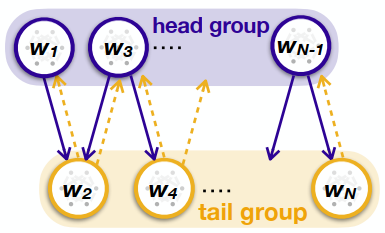
\includegraphics[width=0.5\textwidth,keepaspectratio]{images/GADMM.png}
\end{figure}
{\scriptsize 图片来源:\cite{issaid2020cq-ggadmm} Issaid et al., Communication Efficient Distributed Learning with Censored, Quantized, and Generalized Group ADMM, 2020}

所有的节点被分为了head group $\mathcal{N}_h$ 与tail group $\mathcal{N}_t$,以此来进行交替方向优化。

\end{frame}

%------------------------------------------------
% Page 15

\begin{frame}
\frametitle{GADMM}

于是,要优化的问题变为了
\begin{align*}
    & \text{minimize} \quad \dfrac{1}{N} \sum\limits_{i=1}^N f_i(x_i) \\
    & \text{subject to} \quad x_i = x_{i+1}, \quad i=1,\cdots,N-1
\end{align*}

ADMM循环中的primal updates为
\begin{multline*}
    x_i^{k+1} = \argmin\limits_{x_i} \{ f_i(x_i) + \langle \lambda_{i-1}^k, x_{i-1}^k - x_i \rangle + \langle \lambda_{i}^k, x_{i} - x_{i+1}^k \rangle \\
    + \dfrac{\rho}{2}\lVert x_{i-1}^k - x_i \rVert^2 + \dfrac{\rho}{2}\lVert x_{i} - x_{i+1}^k \rVert^2 \}, \quad i \in \mathcal{N}_h
\end{multline*}
\begin{multline*}
    x_i^{k+1} = \argmin\limits_{x_i} \{ f_i(x_i) + \langle \lambda_{i-1}^k, x_{i-1}^{k+1} - x_i \rangle + \langle \lambda_{i}^k, x_{i} - x_{i+1}^{k+1} \rangle \\
    + \dfrac{\rho}{2}\lVert x_{i-1}^{k+1} - x_i \rVert^2 + \dfrac{\rho}{2}\lVert x_{i} - x_{i+1}^{k+1} \rVert^2 \}, \quad i \in \mathcal{N}_t
\end{multline*}

\end{frame}

%------------------------------------------------
% Page 15

\begin{frame}
\frametitle{CQ-GGADMM}

这一问题随后被推广到了更一般的网络结构上,即从链式的网络结构推广到了一般的二分网络(bipartite graph)上(需要注意的是,这个方案为了进一步降低通信开销,而在local update完成之后进一步对参数采取了quantization以及censoring等手段)。

\begin{figure}[H]
    \centering
    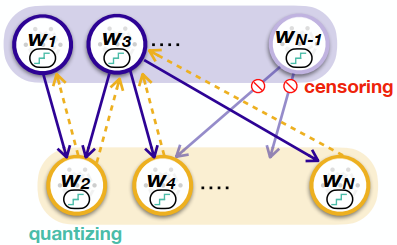
\includegraphics[width=0.5\textwidth,keepaspectratio]{images/CQ-GGADMM.png}
\end{figure}
{\scriptsize 图片来源:\cite{issaid2020cq-ggadmm} Issaid et al., Communication Efficient Distributed Learning with Censored, Quantized, and Generalized Group ADMM, 2020}

\end{frame}

%------------------------------------------------
% Page 15

\begin{frame}
\frametitle{ADMM与神经网络}

待写。。。。

\end{frame}

%------------------------------------------------
% Page 15

% \begin{frame}
% \frametitle{收敛性}



% \end{frame}


% %------------------------------------------------

% \section[Misc]{其他一些问题}  % 其他一些有趣的问题

% %------------------------------------------------
% % Page 15

% \begin{frame}



% \end{frame}

%------------------------------------------------
% Page 15

\begin{frame}[allowframebreaks]
\frametitle{参考文献}

{\footnotesize
\bibliographystyle{ieeetr}
\bibliography{references}
}

\end{frame}

%------------------------------------------------
% Page 15

\begin{frame}
\frametitle{Backup}

Some authors considered a {\color{red} ``weak'' consensus problem} (originally stated as ``mixture'' FL problem)
$$\text{minimize} \quad \sum\limits_{i=1}^N f_i(x_i) + \dfrac{\lambda}{2} \sum\limits_{i=1}^N \lVert x_i - \overline{x} \rVert^2$$
which can be reformulated as constrained optimization problems
\begin{align*}
    & \text{minimize} \quad \sum\limits_{i=1}^N f_i(x_i) + \dfrac{\lambda}{2} \sum\limits_{i=1}^N \lVert x_i - z \rVert^2 \\
    & \text{subject to} \quad Nz - \sum\limits_{i=1}^N x_i = 0
\end{align*}

\end{frame}

%------------------------------------------------
% Page 15

\begin{frame}
\frametitle{Backup}

or equivalently as the following problem,
\begin{align*}
    & \text{minimize} \quad \sum\limits_{i=1}^N f_i(x_i) + \dfrac{\lambda}{2} \sum\limits_{i=1}^N \lVert x_i \rVert^2 -\dfrac{\lambda N}{2} \lVert z \rVert^2 \\
    & \text{subject to} \quad Nz - \sum\limits_{i=1}^N x_i = 0
\end{align*}
which is a nonconvex sharing problem considered in \cite{hong2016convergence} (Eq. (3.2)). Under certain assumptions, this problem is a DC (difference-of-convex) programming problem.

\begin{question}
\begin{itemize}
    \item what is the case when $f_i$ being nonconvex
    \item inexact ADMM iterations (e.g. mini-batch SGD)
\end{itemize}
\end{question}

\end{frame}

%------------------------------------------------
% Page 15

\begin{frame}
\frametitle{Backup}

The original unconstrained problem is studied in \cite{hanzely2020federated} using the so-called loopless local gradient descent (L2GD) method, with the assumptions that
\begin{itemize}
    \item $f_i$ Lipschitz smooth
    \item $f_i$ strongly convex
\end{itemize}

\end{frame}

%------------------------------------------------
% Page 15

\begin{frame}
\frametitle{Backup}

Rewrite $\sum\limits_{i=1}^N f_i(x_i) + \frac{\lambda}{2} \sum\limits_{i=1}^N \lVert x_i - \overline{x} \rVert^2$ as $f(x) + \psi(x)$ with $x = (x_1,\cdots,x_N)$, the local step of L2GD at a client $i$ is
$$x^{k+1} = x^k - \alpha G(x^k)$$
where
$$
G(x^k) = \begin{cases}
\dfrac{\nabla f(x^k)}{1-p} & \text{ with probability } 1-p \\
\dfrac{\lambda \nabla \psi(x^k)}{p} & \text{ with probability } p 
\end{cases}
$$
Locally, one has
$$x_i^{k+1} = x_i^k - \beta \nabla f_i(x_i^k), \quad x_i^{k+1} = (1-\gamma)x_i^k + \gamma \overline{x}^k$$
with probabilities $1-p$ and $p$ respectively.

\end{frame}


%------------------------------------------------

% \begin{frame}

% \Huge{\centerline{\bfseries The End}}

% \vspace{0.5em}

% \Huge{\centerline{\phantom{a}\bfseries 谢谢!}}

% \end{frame}

%------------------------------------------------

\end{document}
